\documentclass{article}
\usepackage{parskip}
\usepackage[margin=1.5cm]{geometry}
\usepackage{graphicx}
\usepackage{framed}
\usepackage{float}
\usepackage{listings}

\graphicspath{{.}}

% Thanks to Angus Pearson for nagging me to fuck about with fonts in
% XeLaTeX

\usepackage{fontspec} \usepackage{xltxtra}

% PT Serif
\setromanfont[ BoldFont=PTF75F.ttf, ItalicFont=PTZ56F.ttf,
BoldItalicFont=PTF76F.ttf, ]{PTF55F.ttf}

% Noto Sans
\setsansfont[ BoldFont=NotoSans-Bold.ttf,
ItalicFont=NotoSans-Italic.ttf, BoldItalicFont=NotoSans-BoldItalic.ttf
]{NotoSans-Regular.ttf}

\begin{document}

\textbf{\Huge Operating Systems Notes}

\section{OSs and Architectures}

Different architectures dictates the way that an operating system must conduct its business.

As different architecture platforms have different instruction sets, it determines what are viable methods for accomplishing tasks such as \textit{memory protection} and \textit{control interrupts}.

The OS acts as an intermediary between software and hardware. It allows to mediate access and gives developers a nicer way of completing lower-level actions. This abstraction is achieved via \textit{traps} and \textit{exceptions}. Similarly, devices can gain attention via the use of \textit{interrupts}.

An OS is intended to be a good balance between \textit{user needs} and \textit{system needs}.

A user wants an OS to be \textit{fast, reliable and safe}; an OS developer wants it to be \textit{efficient, error-free, and easy to maintain and implement}.

The design of an operating systems makes a distinction between two underlying principles:

\textbf{Policy}, which is \textit{what} will be done; \textbf{Mechanism}, which his \textit{how} to do it.

\subsection{Structure of an OS}

A capable operating system is home to a multitude of components: memory management, I/O, file systems, command interpreters and so on. There are multiple ways to link to structure how all these components are connected to each other.

\subsubsection{Monolithic}

An early type of design for an OS, where the \textit{entire} operating system would function in \textit{kernel mode} (see the \textit{Privileged Instructions} section). However, this design carried many issues with maintainability and reliability, and was hard to make sense of.

\subsubsection{Layering}

As opposed to monolithic, this method implemented the OS as a \textit{set of layers} instead, where a layer could present itself to the corresponding layer above.

\begin{figure}[H]
  \centering
  \begin{center}
    \begin{tabular}{|c|c|l|}
      \hline
      5 & \textbf{Job Managers} & Execute a user's programs\\
      \hline
      4 & \textbf{Device Managers} & Handle devices, provide buffering\\
      \hline
      3 & \textbf{Console Manager} & Provide virtual consoles\\
      \hline
      2 & \textbf{Page Manager} & Implement virtual memories for each process\\
      \hline
      1 & \textbf{Kernel} & Implement a virtual processor for each process\\
      \hline
      0 & \textbf{Hardware} & \\
      \hline
    \end{tabular}
  \end{center}
  \caption{Dijkstra's THE System}
\end{figure}

Layering provides a \textit{hierarchical} structure but provides performance issues as overhead increases at each layer. Systems can be modelled as layers, but tend not to be implemented in such a way in reality.

\subsubsection{Hardware Abstraction Layer}

More common in modern OSs. The idea is to have a \textit{core OS}, components such as the file system and scheduler, which don't depend on hardware. Then, you have the \textit{hardware abstraction layer} which specifically deals with the hardware through \textit{drivers} and \textit{assembly routines}.

This allows for more portability, as the layer deals with translation between the core and the specifics of the hardware; developers don't have to worry about specific traits of some hardware and can instead deal with specifics of the core.

\subsubsection{Microkernel}

This concept aims to minimise what the \textit{kernel} is responsible for, and have the rest dealt with by processes at the user level.

This isolation allowed isolation between the components, but provides poor performance as the number of user/kernel crossings greatly increases.

\subsubsection{Loadable Kernel Modules}

Utilised by Linux, this concept has core services within the kernel code itself, and then other modules can be loaded in \textit{dynamically}.

This style avoids some of the issues that come with layering, as it can call any other module. As the loading is dynamic, there is no need for reboots.

\filbreak
\subsection{Privileged Instructions}

These instructions are restricted to use by the OS \textit{only}, and includes direct access to \textit{I/O devices} and \textit{memory state management}.

This is achieved by the implementation of two \textit{modes of operation}; \textit{user} and \textit{kernel} modes.

Privileged instructions can only be executed in kernel mode.

\begin{figure}[h!]
  \centering
  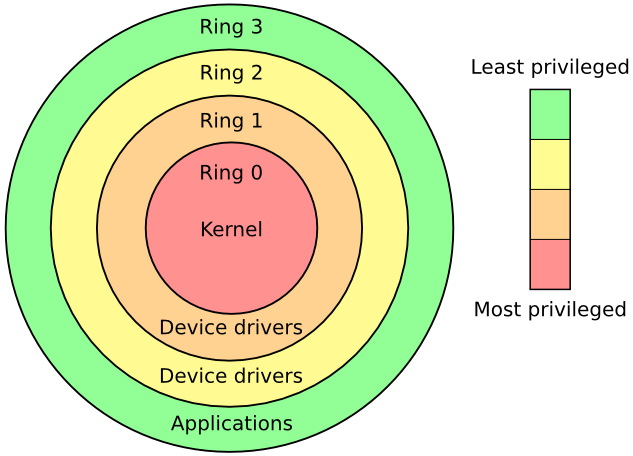
\includegraphics[scale=0.35]{privilegeGraphX86}
  \caption{x86 Architecture Levels of Privilege}
  \textit{\footnotesize Courtesy of Hertzsprung of English Wikipedia}
\end{figure}

\subsubsection{System Calls}

If code running from within user mode tries to execute a privileged instruction, it will trigger the \textit{illegal execution trap}, which allows for such code to gain access to privileged instructions and resources. These are called \textit{system calls}.

An OS will define a set of system calls that makes it possible for such an interaction to take place.

\begin{figure}[H]
  \begin{framed}
    \textit{Caller}: The user mode process invoking the system call\\
    \textit{Callee}: The OS handling the system code\\
    \begin{itemize}
    \item The caller places arguments, especially the \textit{type} of system call, in a specified location
    \item The callee saves the caller's state
    \item The callee verifies the arguments
    \item If valid, the code is run
    \item When the system call has been satisfied, the program counter is set to the return address
    \item Execution is returned to user mode
    \end{itemize}
  \end{framed}
  \caption{A rough breakdown of a system call}
\end{figure}

\subsection{Exception Handling}

A \textit{trap} is a synchronised, intended transition that is initiated by the OS.

An \textit{exception} is also synchronised, however it is an \textit{unexpected} problem with some instruction.

An \textit{interrupt} is \textit{a}synchronous on the other hand, and is caused by some external device.


\filbreak
\section{Threading}

Instead of using multiple processes for concurrency, we can use threads, which share the same address
space and OS resources. This smaller overhead usually results in threads being more performant than
the same number of separate processes.

With threads, we want the same program code, data, privelages and resources (open files, sockets...) but
we need multiple execution states (each thread has it's own registers and stack)

From the perspective of the parent process to a set of threads, the \emph{heap} is shared, and each thread has
it's own \emph{stack pointer} and \emph{PC}.

\subsection{Kernel Threading}

The kernel presents it's own threading library, with the kernel managaing both the process and threads memory.
Kernel threads are more performant than just processes, but because they are handled through \textbf{system calls}
there's still a sizeable overhead.

\subsection{User-Level Threading}

User threads are built completely transparently to the underlying OS, which only sees the parent processes. User
threads can be very performant, though if one thread is blocked due to IO etc., the entire process will also be
blocked as there is no way for the kernel to schedule other threads as it isn't aware of them.

User threads can be 10 to 100 times faster than kernel threads.

A combination of kernel threading and user-space threading can be used to get the best performance.


\filbreak
\subsection{Processes}

A \textit{process} is a program that is being executed.

A process must have a few key aspects for them to work:

\textbf{Address Space}

Contains the \textit{instructions} of the running program, and the \textit{data} for running the program.

\begin{figure}[H]
  \centering
  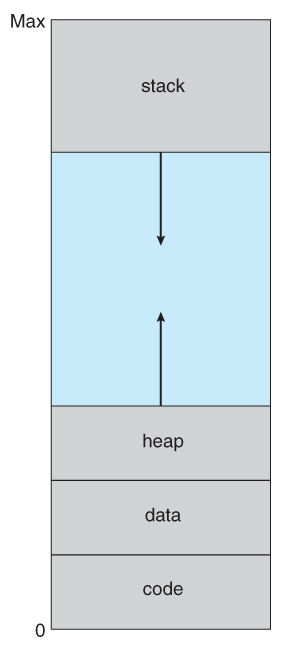
\includegraphics[scale=0.64]{addressspace}
  \caption{An idealised address space given for a process}
\end{figure}

\textbf{CPU State}

Contains the \textit{program counter} which indicates the next instruction, the \textit{stack pointer} and other register values.

\textbf{OS Resources}

Contains items that the OS gives the process access to, such as files, network connections and so on.

\subsection{PCB: Process Control Block}

The operating system needs a way to keep a track of all processes that are running.

A data structure, called the \textit{process control block}, or \textit{process descriptor}, aims to do this.

This name space includes all the \textit{process IDs} of the processes that are currently present. A process ID is a \textit{unique integer}.

A process is called by the \texttt{fork()} function, and can be \textit{killed} (\texttt{kill()}), \textit{paused} (\texttt{wait()}), and \textit{limited} (\texttt{nice()}).

The PCB keeps: the process' \textit{execution state} when the process isn't active; the parent's PID; program counter; and so on. Linux's PCB has over 95 fields for \textit{each} entry.

\subsection{Sequential Process}

The most simple style of process.

A \textit{sequential process} is given some \textit{address space} and a \textit{thread of execution}. The process will then be executed.

\section{Memory Management}
Programs must be brought from disk into mmemory and then placed into a process.

The CPU can only access data from memory, not disk.

Register access takes at most 1 CPU clock, but Main Memory can take mayn cycles, causing a \emph{Stall}.

\subsection{Base and Limit Registers}
A set of \emph{base} and \emph{limit registers} define the logical adress space. the CPU must chech every
memory access is valid between the base and the limit for that user. Failure causes a trap to the OS monitor

\subsection{Virtual Address Space}
Logical/Virtual addresses are independent of physical memory.

Hardware translates virtual addresses into physical ones.

Logical/Virtual addresses a process can reference is called the address space.

\subsection{Memory Managment Unit (MMU)}
Effectively is a hash function from logical address to physical address.

a MMU prevents the need for swapped out process to be swapped back into the same physical addresses.

Swapping is not typically supported on mobile devices, more likely to to overwite least used data.


\subsection{Partitioning}
Main memory is usually broken up into two partitions; The OS and user process.

Each process is contained within a single contiguous section on memory.

Reallocation registers are used to protect users processes from one another and from canging the OS code.

Some old techniques include:
\begin{itemize}
    \item Fixed Partitions - simple but causes fragmentation often
    \item Variable Partitions - no internal fragmentation, but can leave holes in the physical memory
\end{itemize}

Dynamic Storage-Allocation is possible using First-fit, Best-fir and Worst-fit in terms of hole filling.

\section{Virtual Memory}
Paged virtual memory allows larger logical address space than physical memory.
Not all pages of the address space need to be in memory. All needed pages are transfered to free page frames.
If there are no free frames, then we evict one.

\subsection{Page Fault}
If there is a reference to a page that isn't stored in memory, then there will be a trap to the OS, a page fault.

The OS ten finds a free frame, swaps page into frame via a sheduled disk operation then resets the tables for validity.

Pages are only brought into memory when referenced, this is called demand paging.

\subsection{Page Replacement}
There are a couple ways to pick which page to replace.
\begin{itemize}
    \item Pick a page that won't be needed any time soon
    \item Pick a page that hasn't been used in a while
\end{itemize}

The goal of all of this to reduce the fault rate by selecting the best victim page to remove.
Best being one that will never be touched again.

Belady's proof:
"evicting the page that won’t be used for the longest period of time minimizes page fault rate"

\emph{Thrashing} is when the system spends most of its time serving page faults, and little time doing useful things.

This could mean that there is not enough memory oor that the memory is over-commited


\begin{figure}[H]
  \centering
  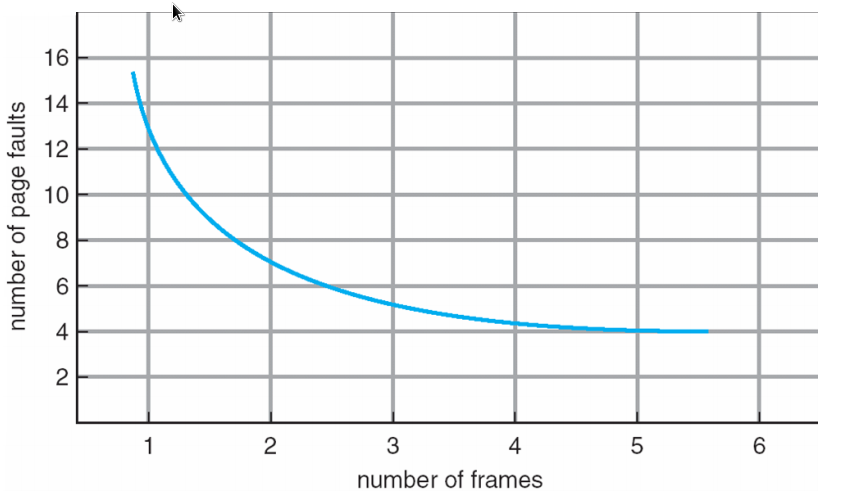
\includegraphics[scale=0.35]{pageFaultGraph.png}
  \caption{Page Faults vs \#Frames}
\end{figure}

\subsubsection{Replacement Algorithms}
\begin{itemize}
    \item First-In-First-Out
    \item Belady's Optimal Algorithm - Replace frame that will not be used for the longest time.
        (Not possible as we can't see into the future)
    \item Least Recently Used(LRU)
    \item Replace a page that is 'old enough' - logically, place all pages in a cirlce and rotate round

\end{itemize}

\vspace{0.5cm}

FIFO and LRU can each be implimented locally or globaly.

Local :- Each process has a limited number of frames and operates within them.

Global :- the vicit is chosen from all page frames in the system, regardless of owner:



\filbreak
\section{MutEx}\label{mutex}

A \emph{critical section} is a sequence of code that may result in
incorrect or undefined behaviour if executed simultaneously or
preempted. Similarly, race conditions occur when the order of execution
is unknown and behaviour can be unpredictable.

Mutual Exclusion (MutEx) and locking prevent these problems.

To be safe and operate correctly, a critical section must satisfy the
following requirements:

\begin{description}
\item[Mutual Exlusion]
At most one thread is in the critical section
\item[Progress]
If a thread is outside the critical section, it cannot prevent another
from entering
\item[Bounded Waiting \& No Starvation]
If a thread is waiting to enter the critical section, it is guaranteed
to eventually do so
\item[Performance]
The overhead of entering and exiting the critical section is small
relative to the runtime of the section.
\end{description}

\begin{figure}[h!]
  \centering
  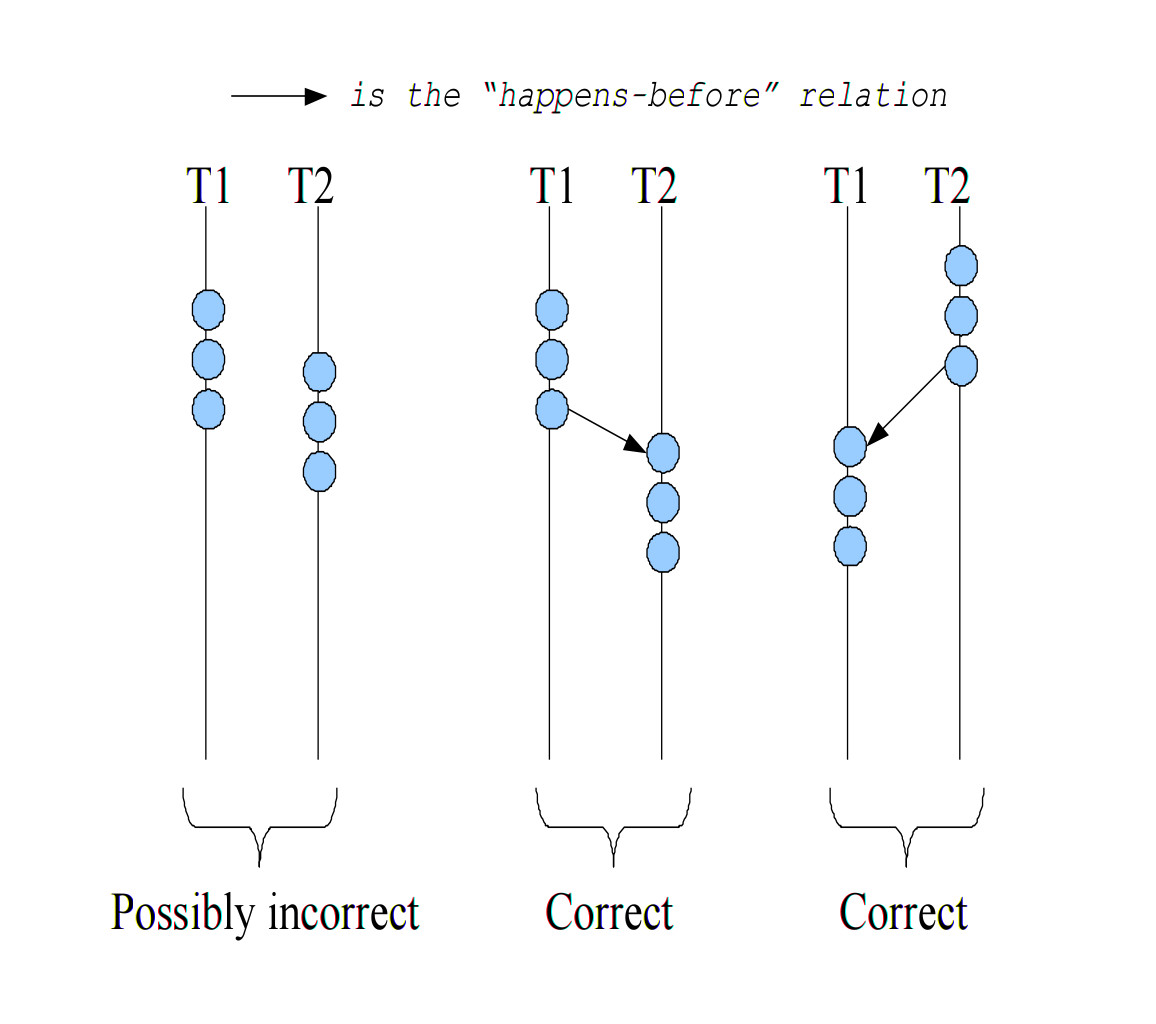
\includegraphics[width=0.5\textwidth]{correctConcurrency}
  \caption{Concurrency Dependencies}
\end{figure}


\subsection{Peterson's Algorithm}\label{petersons-algorithm}

\begin{verbatim}
flag[i] = True;
turn = 1-i;

while (flag[1-i] && turn == 1-i); // spin

/* critical section code */

flag[i] = False;
\end{verbatim}

Avoids both \emph{deadlock} and \emph{livelock} for two threads, using
\texttt{i} and \texttt{i-1} as signals. It works but can be tricky to
implement.

\subsection{Spinlocks}\label{spinlocks}

A \textbf{spinlock} is a locking primative, used to build more complex
locking mechanisms. The name comes from the behaviour; It `spins' on a
condition until it is satisfied, so will acquire the lock as soon as it
is available.

\begin{verbatim}
// do not have lock
while(some_condition);
// have lock
\end{verbatim}

Acquiring and releasing locks \emph{must} be an atomic operation, so no
contect switching occurs during acquisition which could lead to a crash
or undefined state. \textbf{Test and Set} is an atomic instruction we
can use to acheive this.

\begin{verbatim}
struct spinlock{
    int held;
};

struct spinlock lock;
lock.held = 0;

int test_and_set(int* flag){
    int old = *flag;
    flag = 1;
    return old;
}

void acquire(struct lock* lock)
{
    /* This is the `spinning' */
    while(test_and_set(&lock->held));
}

void release(struct lock* lock)
{
    lock->held = 0;
}
\end{verbatim}

Spinlocks are simple to implement, but can be slow and \emph{block}
whilst waiting for the lock, wasting CPU time.

\subsection{Semaphores}\label{semaphores}

Similar to a spinlock, having the two operations
\texttt{wait(semaphore)} and \texttt{signal(semaphore)}, sometimes given
as \texttt{P(semaphore)} and \texttt{V(semaphore)}. Semaphores can use
integer signals, or a boolean - the boolean semaphore has the same
behaviour as a lock.

\begin{verbatim}
void wait(semaphore s)
{
    while(s <= 0); // Busy wait
    s--;
}

void signal(semaphore s)
{
    s++;
}
\end{verbatim}

This simple implementation uses \emph{busy waiting}. We can use a wait
queue instead, placing ourselves onto the queue and yielding until the
semaphore is available.

\begin{verbatim}
void wait(semaphore* s)
{
    s->value--;
    if(s->value < 0){
        enqueue_process();
        /* Add self to the wait queue and block/sleep */
    }
}

void signal(semaphore* s)
{
    s->value++;
    if(s->value <= 0){
        dequeue_process();
        /* Remove a process from the wait queue and wake it */
    }
}
\end{verbatim}

\subsubsection{Bounded Buffer Problem}\label{bounded-buffer-problem}

In a \textbf{producer and consumer} model, we can have many threads
wishing to consume some data, and many that produce it. The handover of
data can be done with a \emph{bounded buffer}

\begin{figure}[h!]
  \centering
  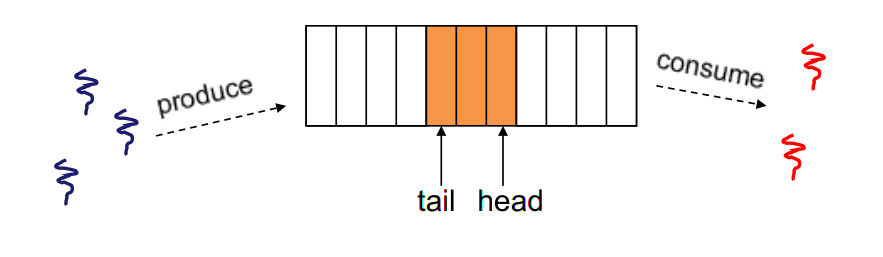
\includegraphics[width=0.8\textwidth]{produceConsume}
  \caption{Producer-Consumer model}
\end{figure}


We can use three semaphores to ensure safety around this bounded buffer:

\begin{tabular}{l | c | l }
mutex & 1 & Mutual exlusion on shared data (head \& tail\ldots{})\\
empty & n & Number of empty / available slots in the buffer. Initially all available.\\
full  & 0 & Number of taken slots in the buffer. Initially none are taken.
\end{tabular}

\begin{verbatim}
producer:
    wait(empty)
    wait(mutex)
        add item to buffer
    signal(mutex)
    signal(full)

consumer:
    wait(full)
    wait(mutex)
        remove item from buffer
    signal(mutex)
    signal(empty)
\end{verbatim}

\subsubsection{Pub Sub}\label{pub-sub}

The constraints on \textbf{publishers} (aka writers) and
\textbf{subscribers} (aka readers) are different:

\begin{enumerate}
\item
  We \emph{can} allow multiple subscribers to concurrently access
\item
  We \emph{cannot} allow publishers and subscribers to concurrently
  access
\item
  We \emph{cannot} have more than one publisher concurrently writing
\end{enumerate}

This is because subscribers make the promise to not mutate the data,
while publishers do not.

\begin{tabular}{l | c | l }
semaphore: mutex     & 1 & Mutual exlusion on shared data\\
semaphore: writing   & 1 & Lock on mutation/writing to the data\\
integer: read\_count & 0 & The number of subscribers currently reading
\end{tabular}

\begin{verbatim}
writer:
    wait(writing)
        perform writes // Satisfies requirement 3
    signal(writing)
    
reader:
    wait(mutex)
        reader_count++;
        if (reader_count == 1) wait(writing); // Satisfy requirement 2
    signal(mutex)
    
    do reading
    
    wait(mutex)
        reader_count--;
        if (reader_count == 0) signal(writing); // Release lock on writers if no further readers
    signal(mutex)
\end{verbatim}

\subsection{Condition Variables}

Has similar operations to Semaphores: \texttt{wait()} and \texttt{signal()}.

\begin{description}
  \item[Wait] Wait until another thread has signaled and released the lock
  \item[Signal] Wake a thread from the wait queue
\end{description}

Signals aren't remembered if there are no threads in the wait queue like they are with semaphores.

\subsubsection{Bounded Buffer}


\begin{tabular}{l | c | l }
lock:      mutex    & 1 & Mutual exlusion on shared data (head \& tail\ldots{})\\
condition: freeslot & n & There is at least one slot free\\
condition: fullslot & 0 & There is at least one slot taken
\end{tabular}

\begin{verbatim}
producer:
    lock(mutex)
    if [no slots available] wait(freeslot);
        Add item...
    signal(fullslot)
    unlock(mutex)

consumer:
    lock(mutex)
    if [no slots have data] wait(fullslot);
        Pop item from shared buffer
    signal(freeslot)
    unlock(mutex)
    Use item...
\end{verbatim}

\subsection{Possible Bugs}

Most locking mechanisms are prone to bugs; They're shared data structures, and there's never a
guarantee a logck will ever be released or acquired when it should be.

The lock is also not strictly associated with the data it protects; Have we got the right lock? 
Should we have more than one lock? Programming language structures
such as classes with built in locking mechanisms go some way to protect against these errors.


\subsection{Monitors}

A higher level programming language structure, requires some notion of objects (so would be tricky 
in C, much easier in C++). Each method in the class automatically acquires a lock on entry, 
releasing it on exit. This is transparent to the implementer of the API exposed by the class. 
Safeties that come from using classes, such as protected/private methods and structures help protect data.

Implementation of a monitor class in C++. \verb|invariant| is asserted over the life of a class, throwing an
error if the condition is broken. Similarly \verb|precondition| asserts a condition before method
execution is allowed. 

\begin{verbatim}
class Account {
  private lock myLock;

  private int balance := 0
  invariant balance >= 0

  public method boolean withdraw(int amount)
     precondition amount >= 0
  {
    myLock.acquire();
    try:
      if balance < amount then return false
      else { balance := balance - amount ; return true }
    finally:
      myLock.release();
  }

  public method deposit(int amount)
     precondition amount >= 0
  {
    myLock.acquire();
    try:
      balance := balance + amount
    finally:
      myLock.release();
  }
}
\end{verbatim}
\emph{Hoiked from wikipedia, https://en.m.wikipedia.org/wiki/Monitor\_(synchronization)}

\end{document}
